\documentclass{article}
\usepackage{graphicx}
\usepackage[margin=1.5cm]{geometry}
\usepackage{amsmath}

\begin{document}

\title{Tuesday Reading Assessment: Chapter 2,3}
\author{Prof. Jordan C. Hanson}

\maketitle

\section{Bit Parity, Error Checking (ch. 2)}

\begin{enumerate}
\item Observe Fig. \ref{fig:par} below, depicting the 4-bit BCD code.  Observe how the parity bit causes \textit{even} parity (even number of 1's), or \textit{odd} parity (odd number of 1's).  Circle all the following 4-bit BCD code words below that have a \textit{single-bit} error, assuming the parity bit is even:
\begin{itemize}
\item 100110010
\item 011101010
\item 10111111010001010
\end{itemize}
\begin{figure}[ht]
\centering
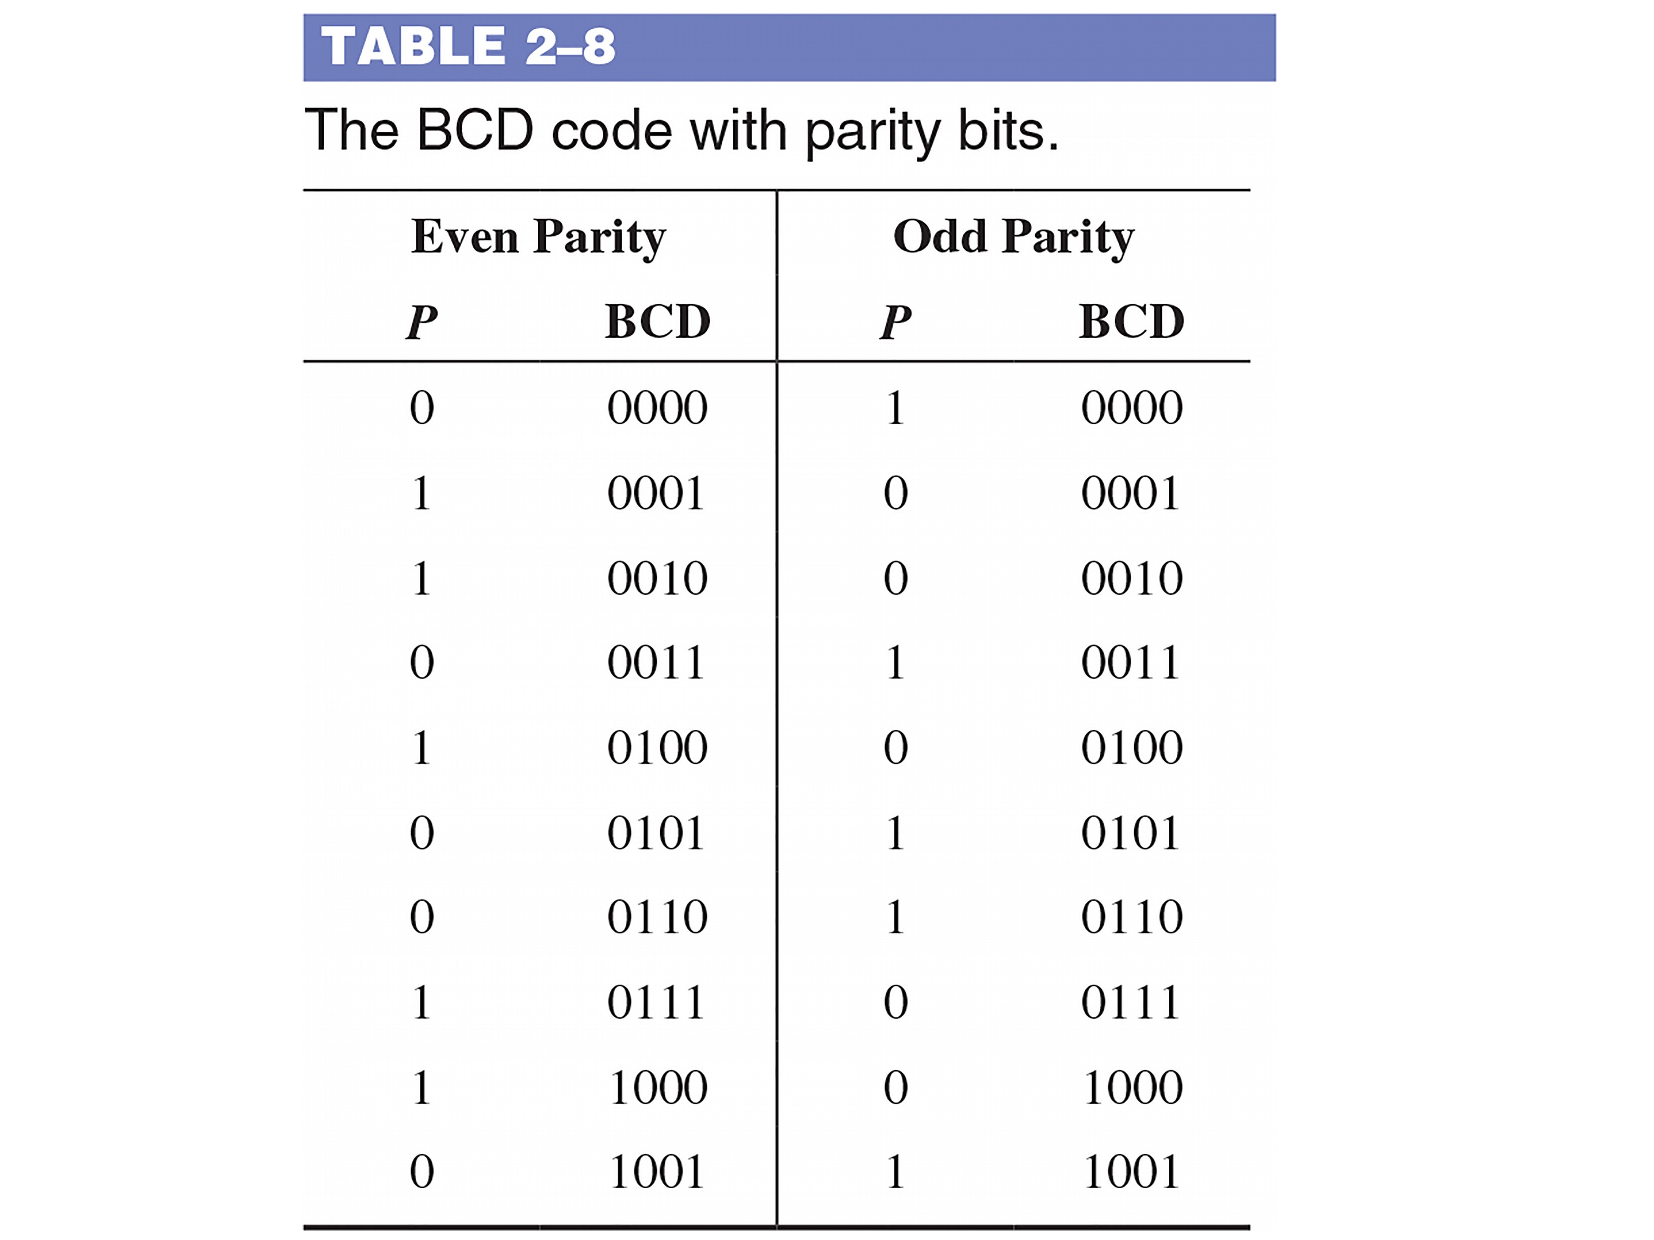
\includegraphics[width=0.3\textwidth]{parity.pdf}
\caption{\label{fig:par} Three basic logic operations.}
\end{figure}
\item Same question, but the parity bit is \textit{odd}:
\begin{itemize}
\item 11110110
\item 00110001
\item 01010101010101010
\end{itemize}
\end{enumerate}

\section{Basic Logic Gates (ch. 3)}

\begin{enumerate}
\item Draw the proper timing diagram for the 4-input AND gate below.  \textit{Hint: what should the truth table be for the 4-input AND?}
\begin{figure}[ht]
\centering
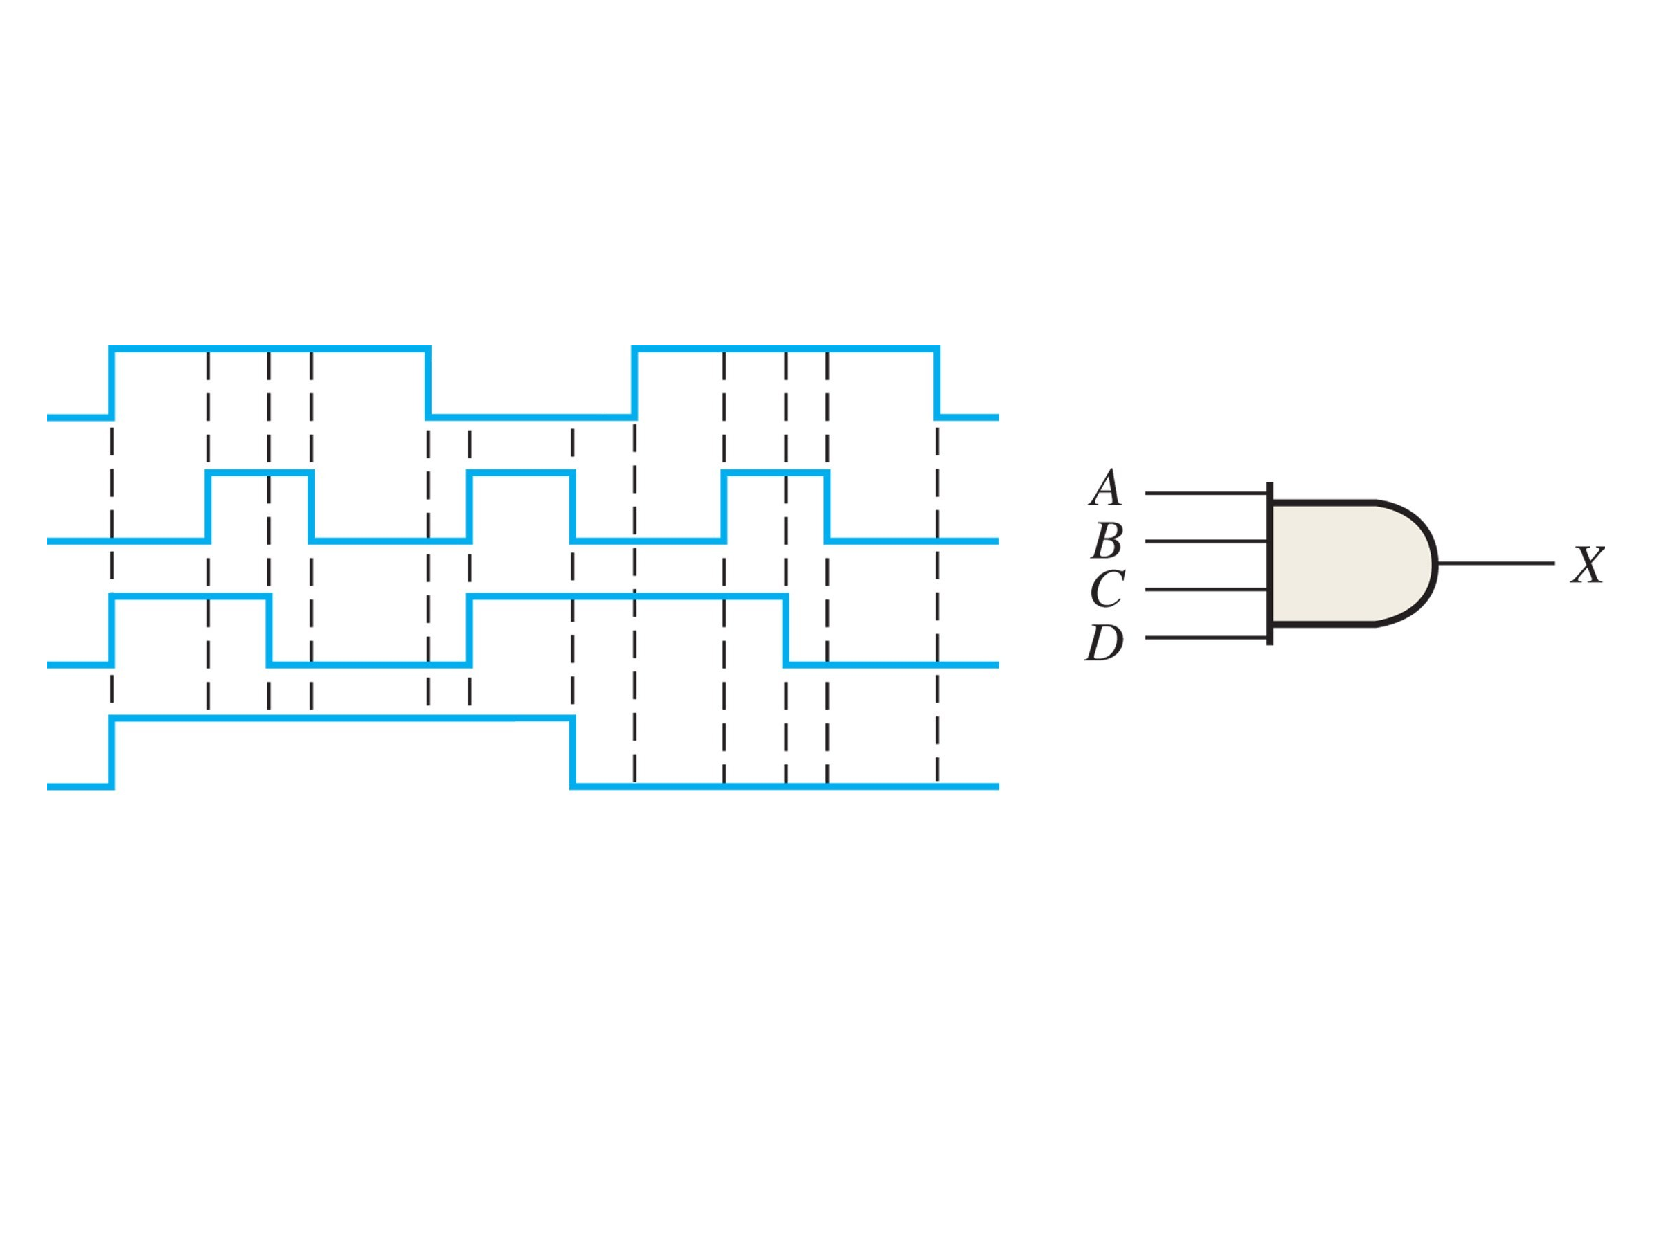
\includegraphics[width=0.4\textwidth,trim=0cm 4cm 0cm 4cm,clip=true]{4and.pdf}
\caption{\label{fig:4and} Three basic logic operations.}
\end{figure}
\end{enumerate}

\end{document}
